%%%%%%%%%%%%%%%%%%%%%%%%%%%%%%%%%%%%%%%%%
% Beamer Presentation
% LaTeX Template
% Version 1.0 (10/11/12)
%
% This template has been downloaded from:
% http://www.LaTeXTemplates.com
%
% License:
% CC BY-NC-SA 3.0 (http://creativecommons.org/licenses/by-nc-sa/3.0/)
%
%%%%%%%%%%%%%%%%%%%%%%%%%%%%%%%%%%%%%%%%%

%----------------------------------------------------------------------------------------
%	PACKAGES AND THEMES
%----------------------------------------------------------------------------------------

\documentclass{beamer}

\mode<presentation> {

% The Beamer class comes with a number of default slide themes
% which change the colors and layouts of slides. Below this is a list
% of all the themes, uncomment each in turn to see what they look like.

%\usetheme{default}
%\usetheme{AnnArbor}
%\usetheme{Antibes}
%\usetheme{Bergen}
\usetheme{Berkeley}
%\usetheme{Berlin}
%\usetheme{Boadilla}
%\usetheme{CambridgeUS}
%\usetheme{Copenhagen}
%\usetheme{Darmstadt}
%\usetheme{Dresden}
%\usetheme{Frankfurt}
%\usetheme{Goettingen}
%\usetheme{Hannover}
%\usetheme{Ilmenau}
%\usetheme{JuanLesPins}
%\usetheme{Luebeck}
%\usetheme{Madrid}
%\usetheme{Malmoe}
%\usetheme{Marburg}
%\usetheme{Montpellier}
%\usetheme{PaloAlto}
%\usetheme{Pittsburgh}
%\usetheme{Rochester}
%\usetheme{Singapore}
%\usetheme{Szeged}
%\usetheme{Warsaw}

% As well as themes, the Beamer class has a number of color themes
% for any slide theme. Uncomment each of these in turn to see how it
% changes the colors of your current slide theme.

%\usecolortheme{albatross}
%\usecolortheme{beaver}
%\usecolortheme{beetle}
%\usecolortheme{crane}
%\usecolortheme{dolphin}
%\usecolortheme{dove}
%\usecolortheme{fly}
%\usecolortheme{lily}
%\usecolortheme{orchid}
%\usecolortheme{rose}
%\usecolortheme{seagull}
%\usecolortheme{seahorse}
%\usecolortheme{whale}
\usecolortheme{wolverine}

%\setbeamertemplate{footline} % To remove the footer line in all slides uncomment this line
%\setbeamertemplate{footline}[page number] % To replace the footer line in all slides with a simple slide count uncomment this line

%\setbeamertemplate{navigation symbols}{} % To remove the navigation symbols from the bottom of all slides uncomment this line
}

\usepackage{graphicx} % Allows including images
\usepackage{booktabs} % Allows the use of \toprule, \midrule and \bottomrule in tables

% Usar lenguaje y letras españolas

\usepackage[spanish]{babel}
\selectlanguage{spanish}
\usepackage[utf8]{inputenc}

%----------------------------------------------------------------------------------------
%	TITLE PAGE
%----------------------------------------------------------------------------------------

\title[Miracast]{Miracast y Google cast} % The short title appears at the bottom of every slide, the full title is only on the title page

\author{Adrián Orduña Díaz,\\ Rafael Leyva Ruiz} % Your name
\institute[UGR] % Your institution as it will appear on the bottom of every slide, may be shorthand to save space
{
Universidad de Granada \\ % Your institution for the title page
\medskip
\textit{rafaelleru95103@correo.ugr.es \\
adrianod@correo.ugr.es} % Your email address
}

\date{\today} % Date, can be changed to a custom date

\begin{document}

\begin{frame}
\titlepage % Print the title page as the first slide
\end{frame}
\begin{frame}
\frametitle{Overview} % Table of contents slide, comment this block out to remove it
\tableofcontents % Throughout your presentation, if you choose to use \section{} and \subsection{} commands, these will automatically be printed on this slide as an overview of your presentation
\end{frame}

%----------------------------------------------------------------------------------------
%	PRESENTATION SLIDES
%----------------------------------------------------------------------------------------

%------------------------------------------------
\section{Introducción sobre Miracast} % Sections can be created in order to organize your presentation into discrete blocks, all sections and subsections are automatically printed in the table of contents as an overview of the talk



%------------------------------------------------

%\subsection{Subsection Example} % A subsection can be created just before a set of slides with a common theme to further break down your presentation into chunks

\begin{frame}
  \frametitle{Breve descripcion de Miracast}
Miracast es una tecnología licenciada por la WiFi Alliance que permite hacer streaming de contenido desde
dispositivos moviles a reproductores compatibles.\\

¡¡Podemos transmitir la pantalla de nuestro movil a la tele!!
\end{frame}

%------------------------------------------------
\begin{frame}
  \frametitle{Ejemplos de uso}
  \begin{itemize}
    \pause
  \item Permite hacer mirroring desde una pantalla a otra
    \pause
  \item Emision de contenidos en streaming sin necesidad de conexión a internet.
    \pause
  \item Mostrar una presentacion en una sala de juntas sin cables de por medio.
    \pause
  \item Reproducir musica en altavoces compatibles.
    \pause
  \item Podriamos incluso ver esta presentacion si el proyector no fuese del año 3000 a.C.
  \end{itemize}
\end{frame}

%------------------------------------------------
\begin{frame}
  \frametitle{¿Cuando aparece Miracast?}
  Miracast fue presentado en el CES de las vegas en 2013 y tuvo una gran acogida en el mundo de la electronica de consumo.\\
  Al año siguiente era doportado oficialmente por Android como respuesta al AirPlay de apple. Fue el autentico boom de esta tecnología.
\end{frame}

%------------------------------------------------
\begin{frame}
  \frametitle{Objetivos de Miracast}
  Miracast al igual que otras muchas tecnologías busca brindarnos un furuto sin cables.\\
  El objetivo es que compartir cualquier tipo de contenio con varias personas sea mucho mas facil.
\end{frame}

%------------------------------------------------
\section{Que hay detras de miracast}

\begin{frame}
  \frametitle{Desmontemos miracast}
  Miracast ofrece un mundo sin cables, en el que enseñar una simple foto a la familia es muy sencillo pero
  ¿cómo se consigue eso?\\

  La respuesta es sencilla, aglutinando un gran numero de componentes tecnológicos y proporcionando un acapa de
  abstracción para todo el que quiera emplear la tecnología.
\end{frame}

%------------------------------------------------
\begin{frame}
  \frametitle{Protocolos de Miracast}
  Para llevar a cabo todo su trabajo miracast se apoya en las siguientes tecnologias:

  //hacer tabla aqui
\end{frame}

%------------------------------------------------
\begin{frame}
  \frametitle{Conexión entre dispositivos}
  \begin{itemize}
  \item Emisor se convierte en el primer Host de una LAN.
    \pause
  \item Receptor encuentra la red y envia petición (Normalmente WPS).
    \pause
  \item Emisor acepta o rechaza la peticion.
    \pause
  \item Si el emisor acepta comienza a transmitir contenido a la red P2P.
  \end{itemize}
\end{frame}

%------------------------------------------------
\begin{frame}
  \frametitle{Que es la red P2P}
  Para transmitir el contenido Miracast se basa en la tecnología WiFi direct, la cual crea una red P2P entre todos los
  dispositivos conectados mediante la cual pueden compartir archivos sin necesitad de conexión a internet.
\end{frame}

%------------------------------------------------
\section{WiFi Direct}
\begin{frame}
  \frametitle{WiFi Direct}
  WiFi Direct es una tecnología similar al bluetooth, que perimite la transmision de archivos entre dispositivos, pero que presenta algunas ventajas:

  \begin{itemize}
    \pause
  \item No todos los dispositivos de la red tienen que soportar WiFi Direct.
    \pause
  \item Mayor velocidad de transferencia que Bluetooth 4.0.
    \pause
  \item Mucho mas extensible.
  \end{itemize}
\end{frame}

%------------------------------------------------
\begin{frame}
  \frametitle{Proceso de conexion y transmision de WiFi Direct}
  El proceso de transmision de un archivo por medio de WiFi Direct es el siguiente:

  \pause
  \begin{itemize}
  \item El primer dispositivo de la red se establece como Soft Host.
      \pause
    \item Establece un mecanismo de consultas de modo que todos los que quieran conectarse le preguntan a el.
      \pause
    \item Los demas dispositivos se conectan con una peticion WPS.
      \pause
    \item Comienza la transmision de ficheros mediante FTP o UDP.
  \end{itemize}
\end{frame}
    
    

%------------------------------------------------
\begin{frame}
  \frametitle{Otras caracteristicas de WiFi Direct}
  \begin{itemize}
  \item Acceso a redes corporativas seguras.
    \pause
  \item Cifrado en las conexiones WPA2.
    \pause
  \item Es un posible reemplazo al bluetooth.
  \end{itemize}
\end{frame}

%------------------------------------------------.

\section{Otras caracteristicas de Miracast}
\begin{frame}
  \frametitle{Proteccion de contenidos con derechos de autor}
  Miracast soporta y protege el contenido con copyright, de modo que dificulta la pirateria. Para ello se hace una comprobacion periodica en el emisor, ademas el receptor debe estar preparado para este tipo de contenido, ya que es desencriptado tras su transmision.
\end{frame}

%------------------------------------------------
\begin{frame}
  \frametitle{DHCP}
  La seguridad para este tipo de contenidos la aporta DHCP, el cual garantiza que el receptor evita los intentos de copia ilegitimos.\\
  El emisor cifra una parte del contenido y solo si el emisor tiene la correspondiente certificacion sera capaz de descifrarlo, en otro caso no lo emitirá con toda la calidad posible.
\end{frame}

%------------------------------------------------
\begin{frame}
  \frametitle{Ilustración del proceso de DHCP}
  \begin{figure}[ht]
    \centering
    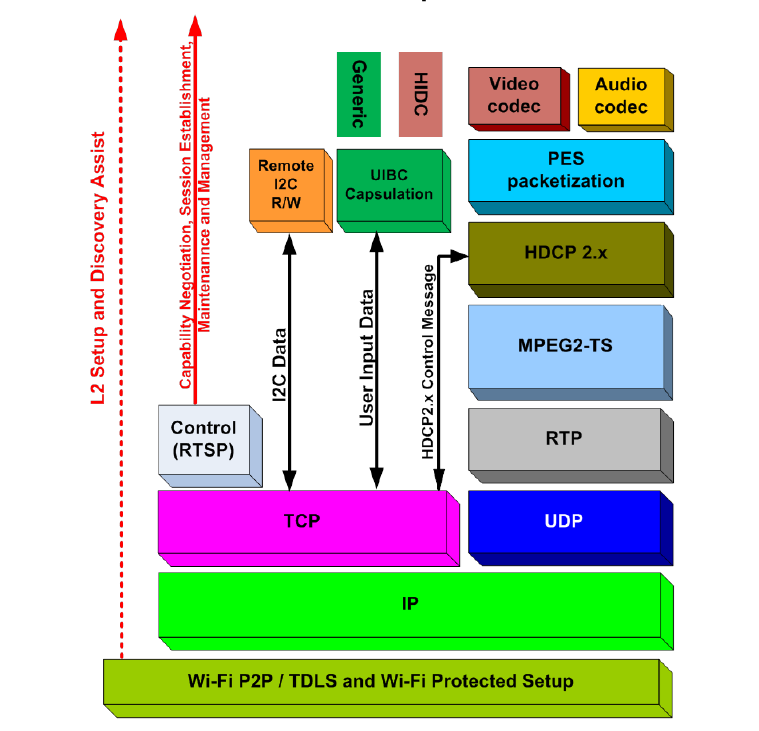
\includegraphics[width=0.65\textwidth]{./Imagenes/HDCP_miracast_layers.png}
    \caption{Esquema de las comunicaciones entre distintas capas de Miracast}
  \end{figure}
\end{frame}

%------------------------------------------------
\section{Demostración de uso y capturas de wireshark}

\begin{frame}
  \frametitle{Mirroring con chromecast usando Miracast}
  Aquí podemos ver como se consigue transmitir la pantalla de nuestro portatil a una pantalla externa sin cables (Aunque no lo parezca):

  \begin{figure}[ht]
    \centering
    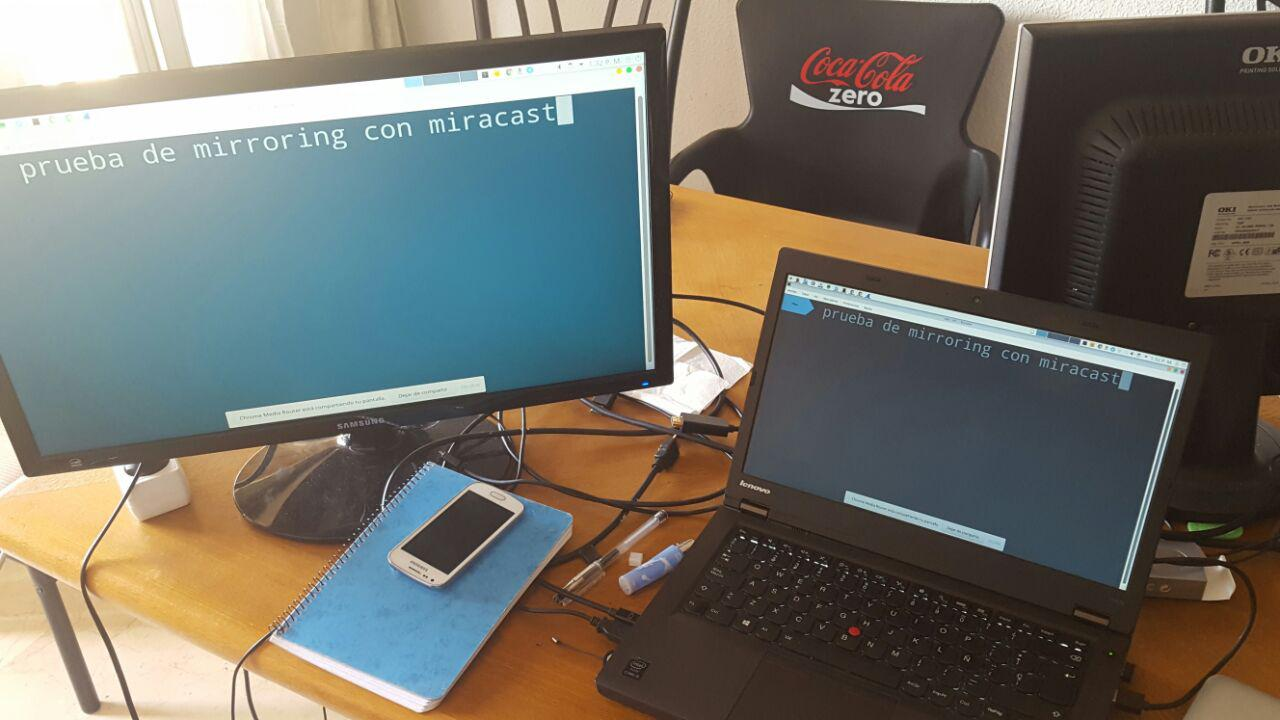
\includegraphics[width=0.8\textwidth]{./Imagenes/CapturaChromecast.png}
    \caption{Foto de Mirroring PC-Google Chromecast}
  \end{figure}
\end{frame}


\begin{frame}
  \frametitle{Captura de datos de la transmision de Miracast con wireshark}
  \begin{figure}
    \centering
    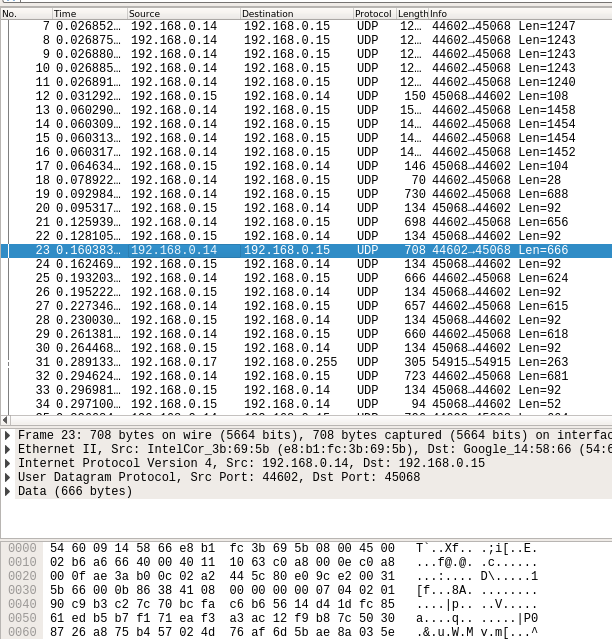
\includegraphics[width=0.7\textwidth]{./Imagenes/wiresarkMiracast.png}
    \caption{Captura de la transmision de datos de Miracast}
  \end{figure}
\end{frame}


%------------------------------------------------
\section{Ruegos y preguntas}

\begin{frame}
  \frametitle{Preguntas}
  Si teneis alguna pregunta este es el momento.
  \end{frame}


\begin{frame}
  \frametitle{Agradecimientos}
  \centering
  Muchas gracias por la atención, perdon por el tostón y muchas gracias.\\

  (Aplausos)
\end{frame}


\end{document}
















